%
\hsection{Installing PgModeler under Ubuntu Linux}%
%
\begin{figure}%
\centering%
%
\subfloat[][%
Open a \bash\ \pgls{terminal} via \ubuntuTerminal. %
Type in \bashil{sudo apt-get install pgmodeler} and hit~\keys{\return}.%
\label{fig:installingPgmodelerUbuntu01aptGetInstall}%
]{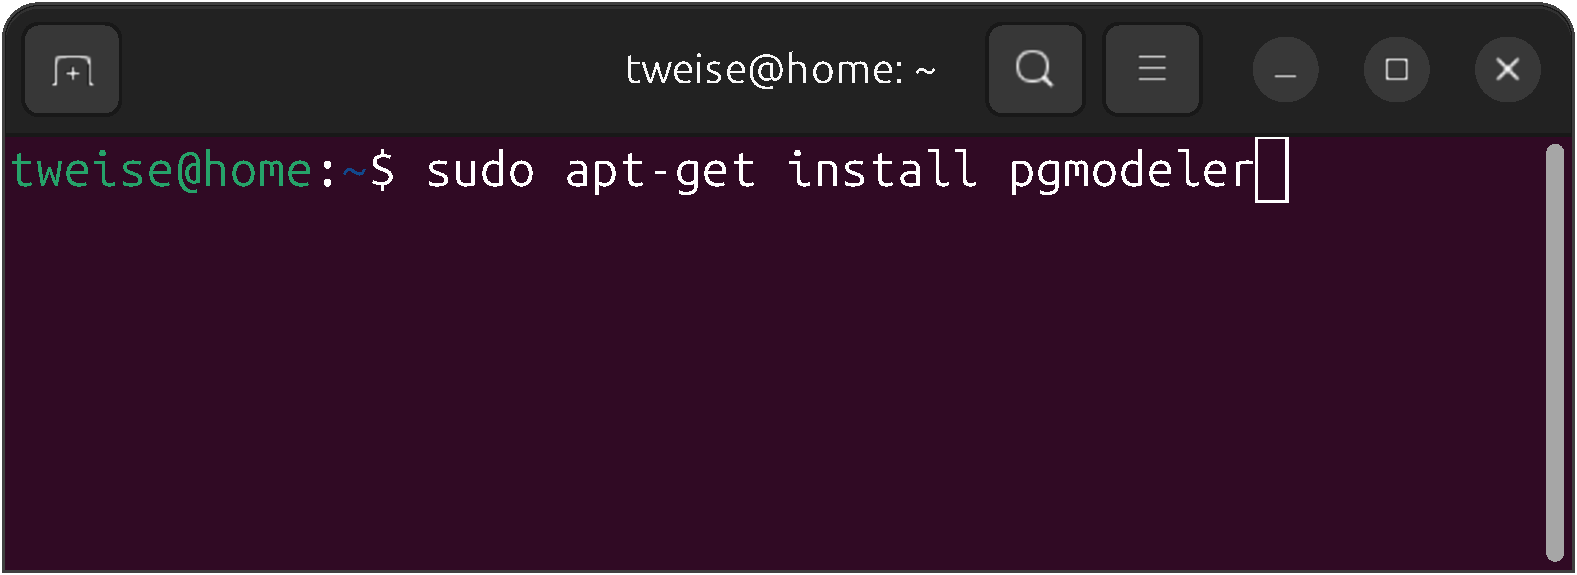
\includegraphics[width=0.7\linewidth]{\currentDir/installingPgmodelerUbuntu01aptGetInstall}}%
%
\floatRowSep%
%
\subfloat[][%
We get asked for the \pgls{sudo} password, type it in, and hit~\keys{\return}.%
\label{fig:installingPgmodelerUbuntu02pw}%
]{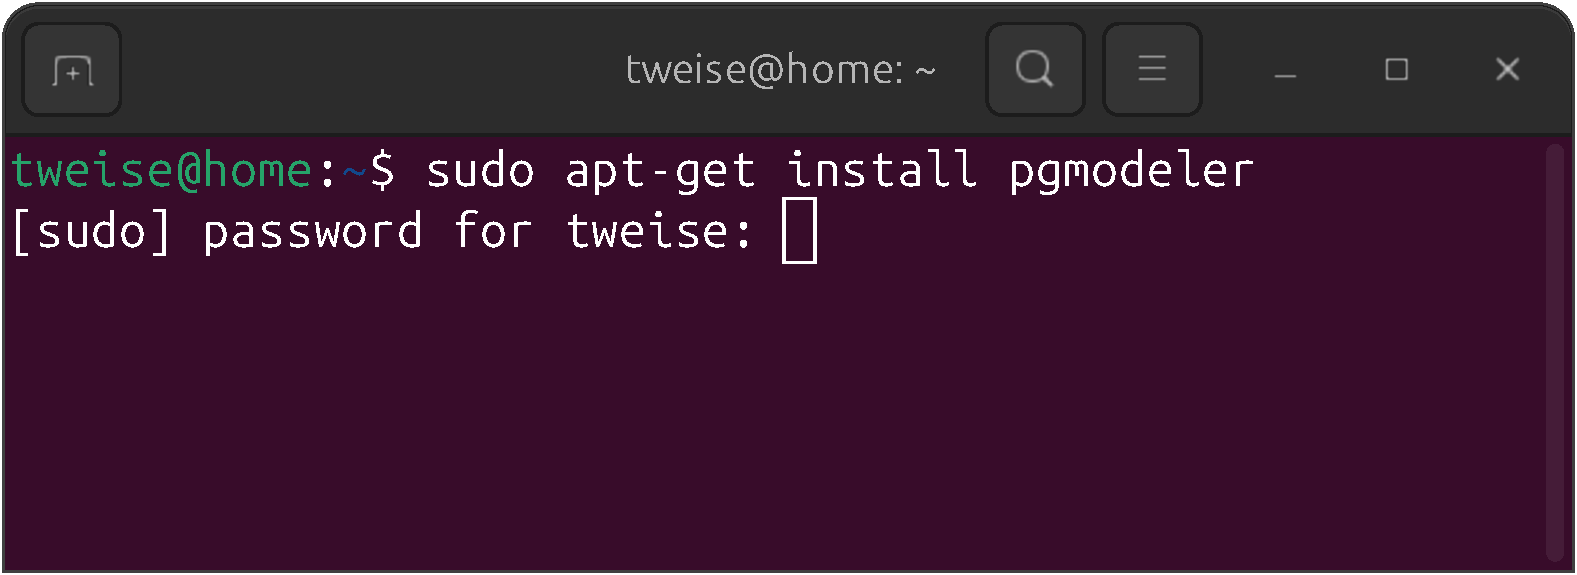
\includegraphics[width=0.7\linewidth]{\currentDir/installingPgmodelerUbuntu02pw}}%
%
\floatRowSep%
%
\subfloat[][%
The system tells us the packages that need to be installed and asks us whether we are OK with that. %
We type~\keys{Y} and hit~\keys{\return}.%
\label{fig:installingPgmodelerUbuntu04yny}%
]{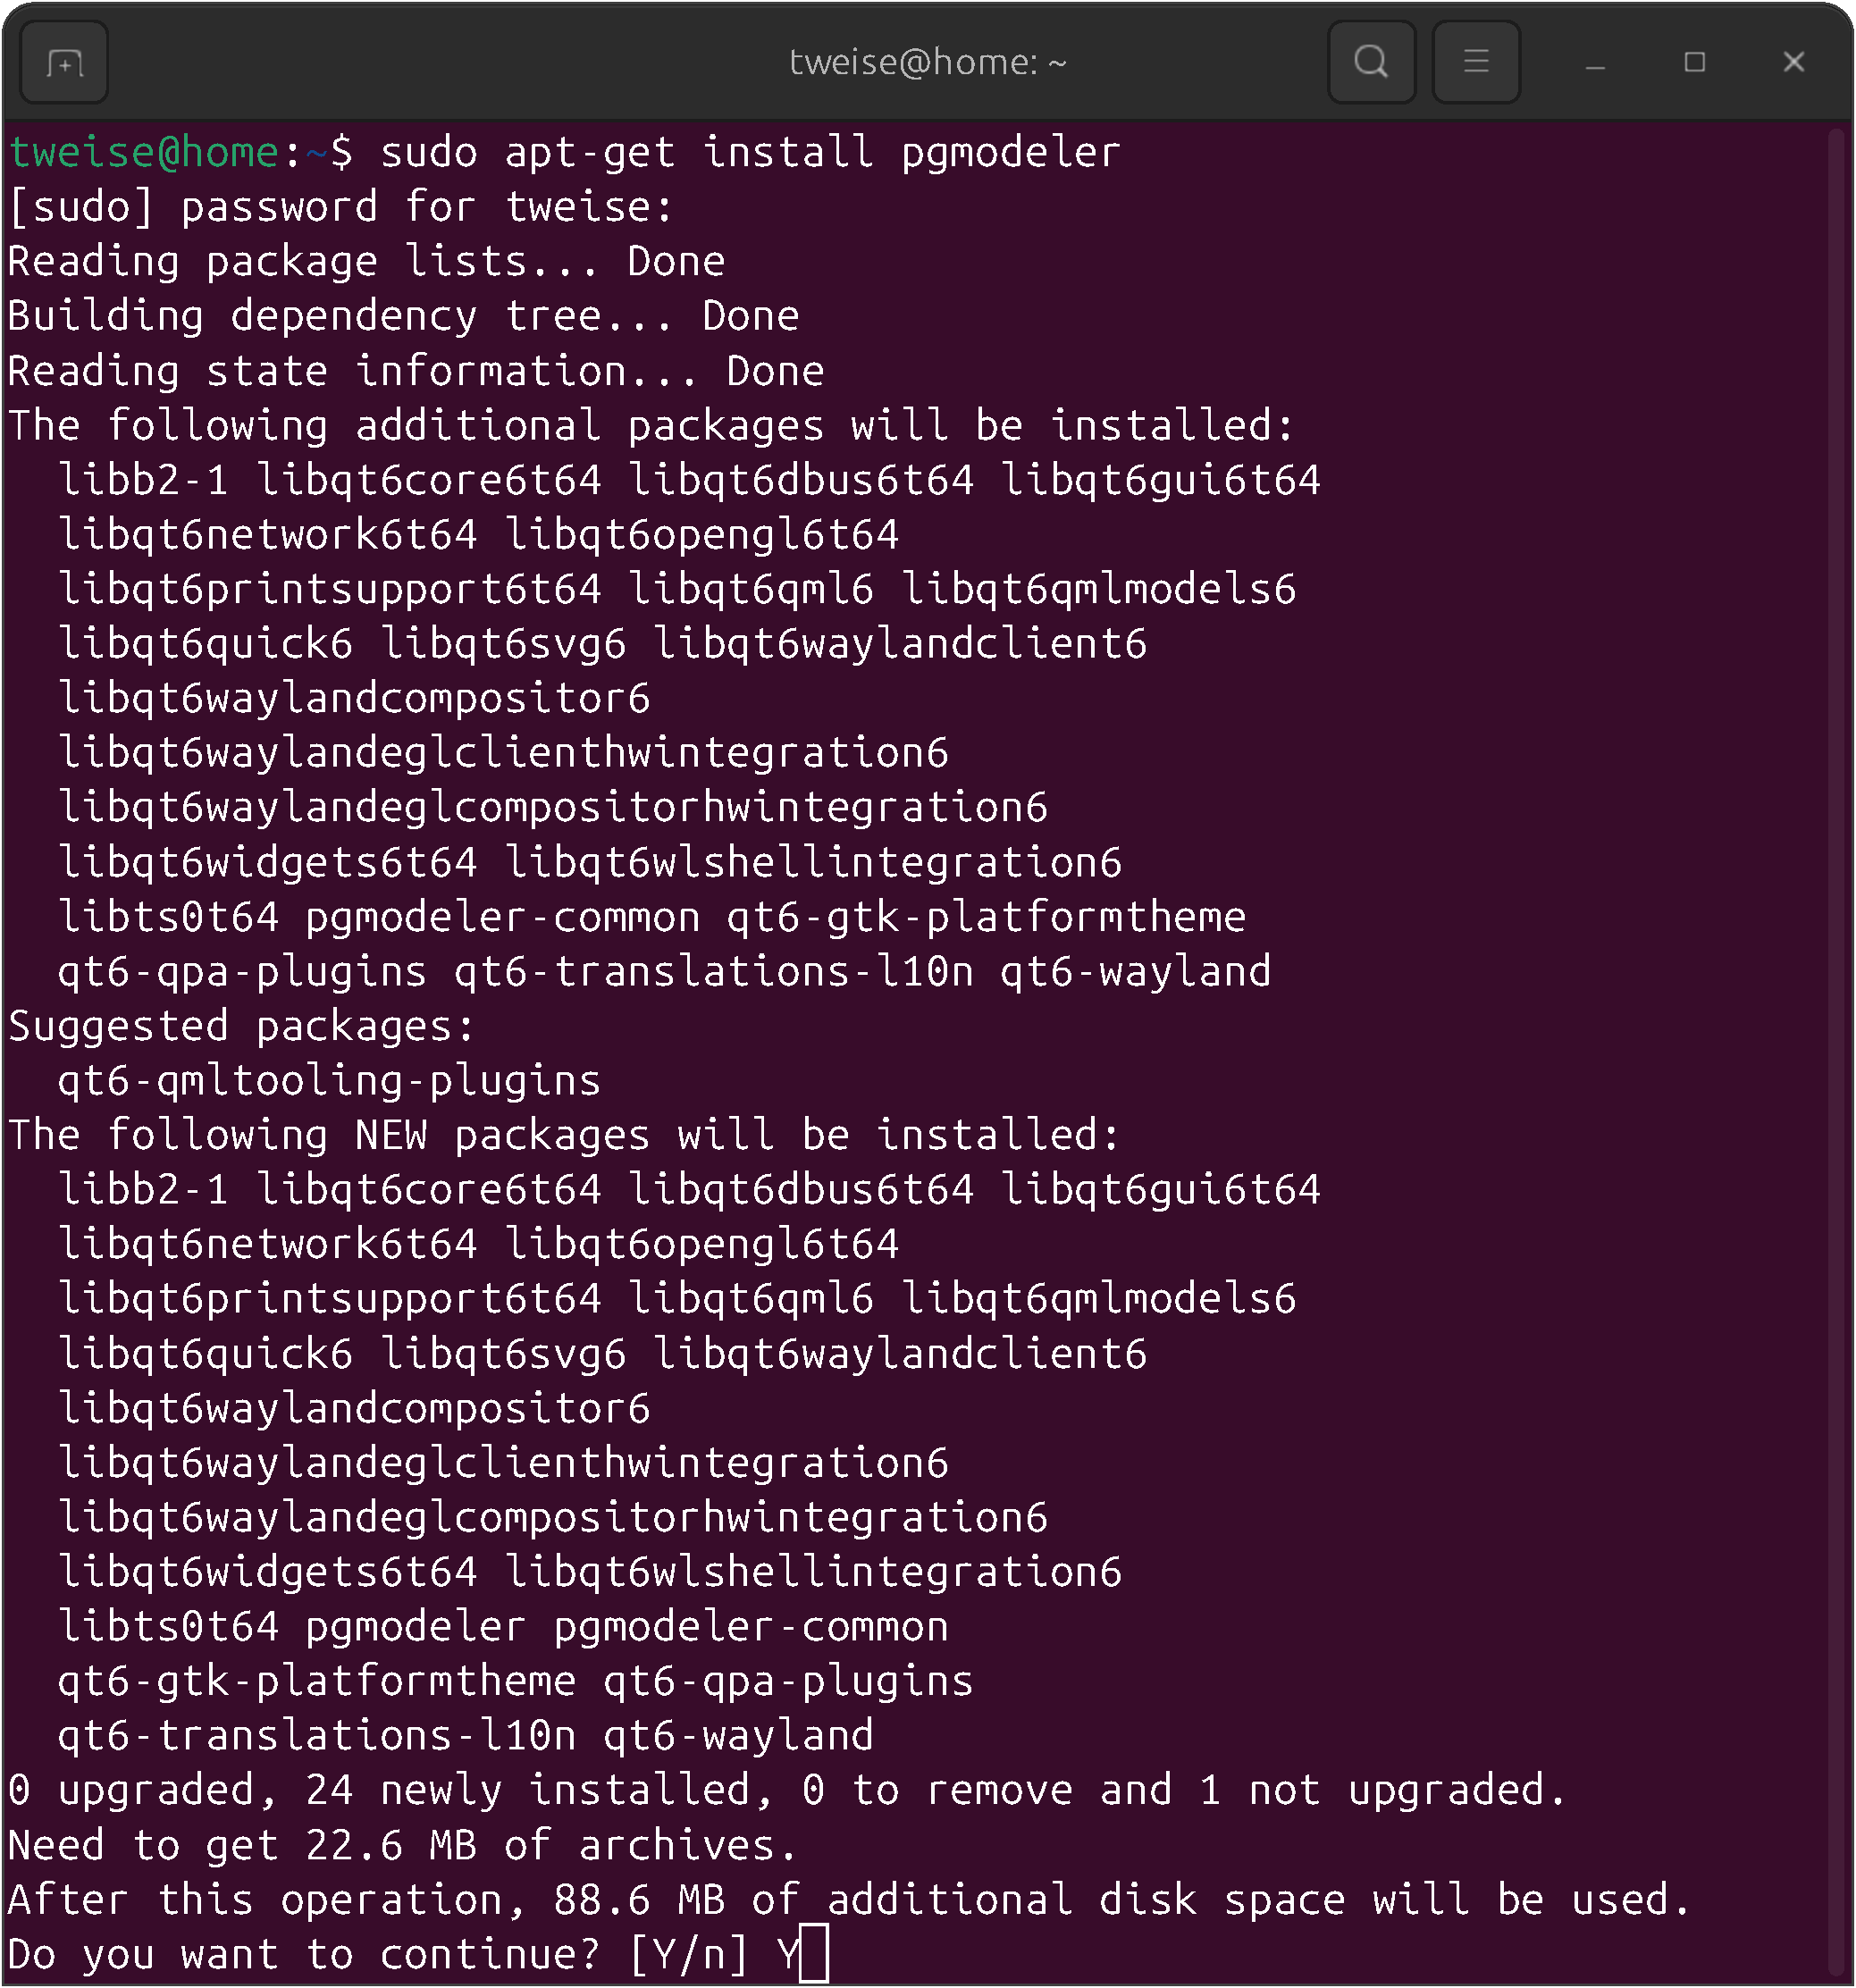
\includegraphics[width=0.7\linewidth]{\currentDir/installingPgmodelerUbuntu04yny}}%
%
\caption{The installation steps for \pgmodeler\ under \ubuntu\ \linux.}%
\label{fig:installingPgmodelerUbuntu:A}%
\end{figure}%
%
\begin{figure}%
\ContinuedFloat%
\centering%
%
\subfloat[][%
The \pgmodeler\ gets installed.%
\label{fig:installingPgmodelerUbuntu05installed}%
]{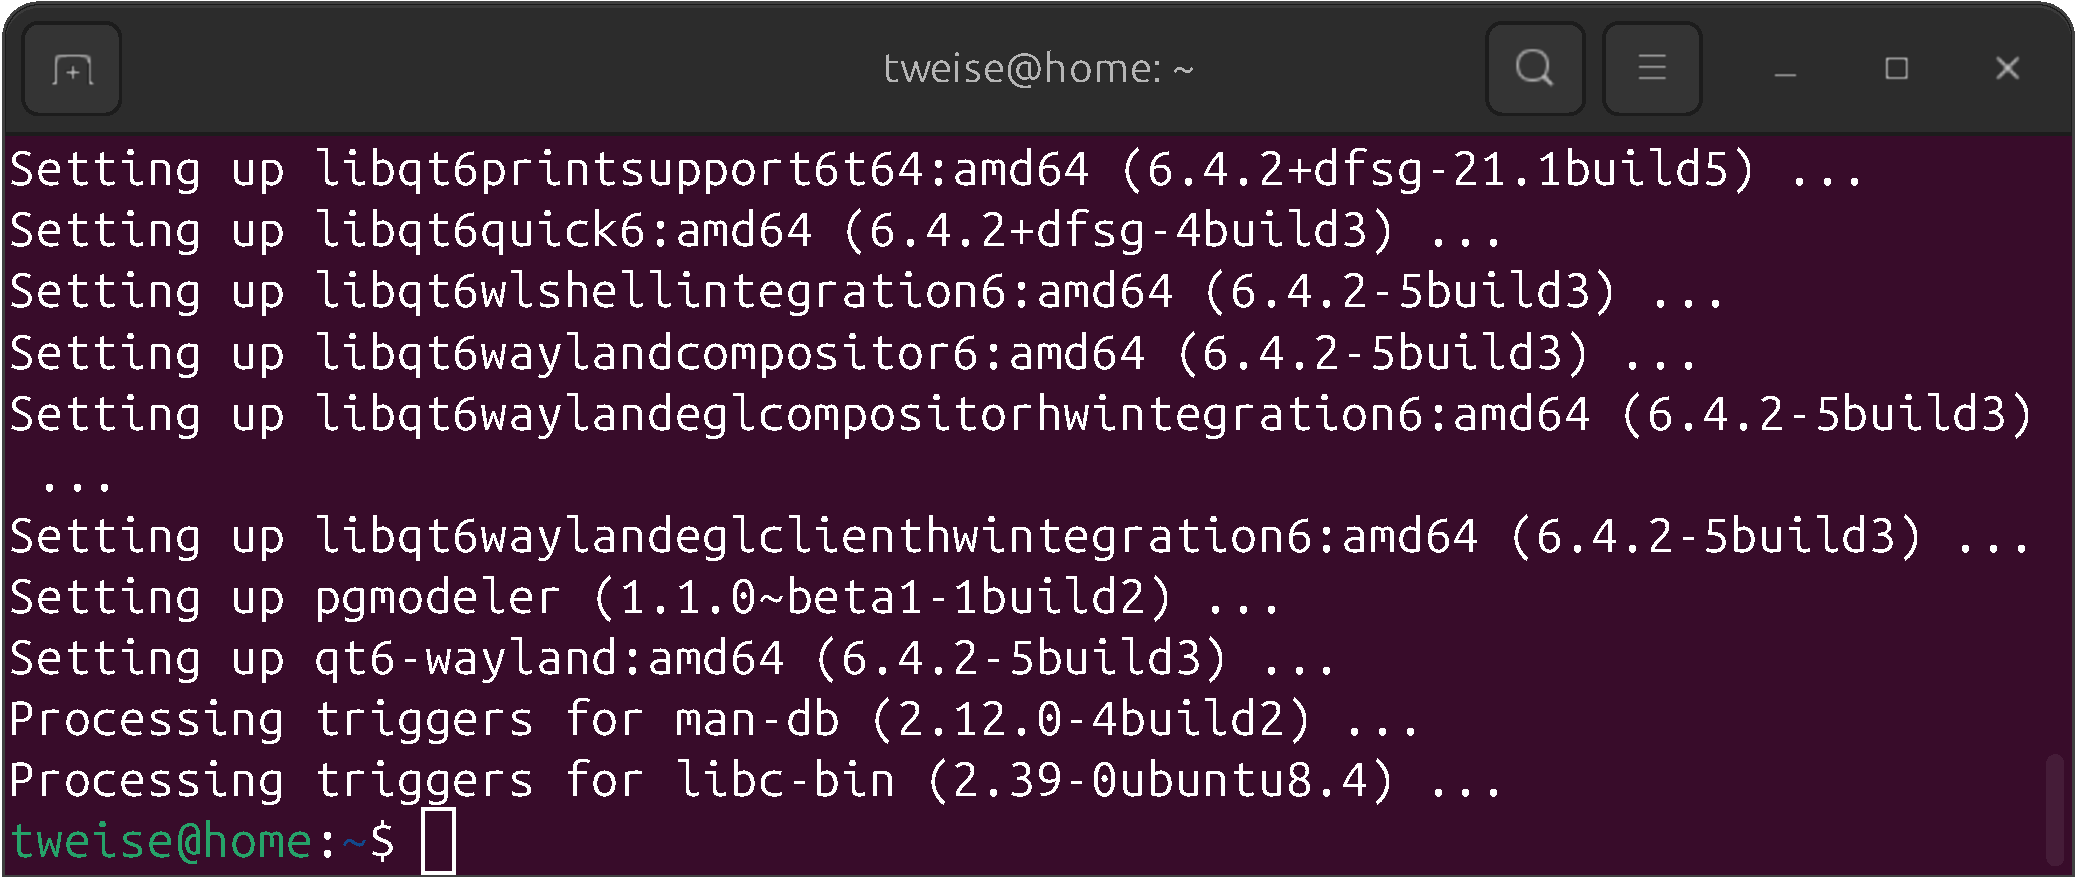
\includegraphics[width=0.7\linewidth]{\currentDir/installingPgmodelerUbuntu05installed}}%
%
\floatRowSep%
%
\subfloat[][%
We now run the \pgmodeler\ by typing \bashil{pgmodeler} into the \bash\ \pgls{terminal} and hitting~\keys{\return}.%
\label{fig:installingPgmodelerUbuntu06run}%
]{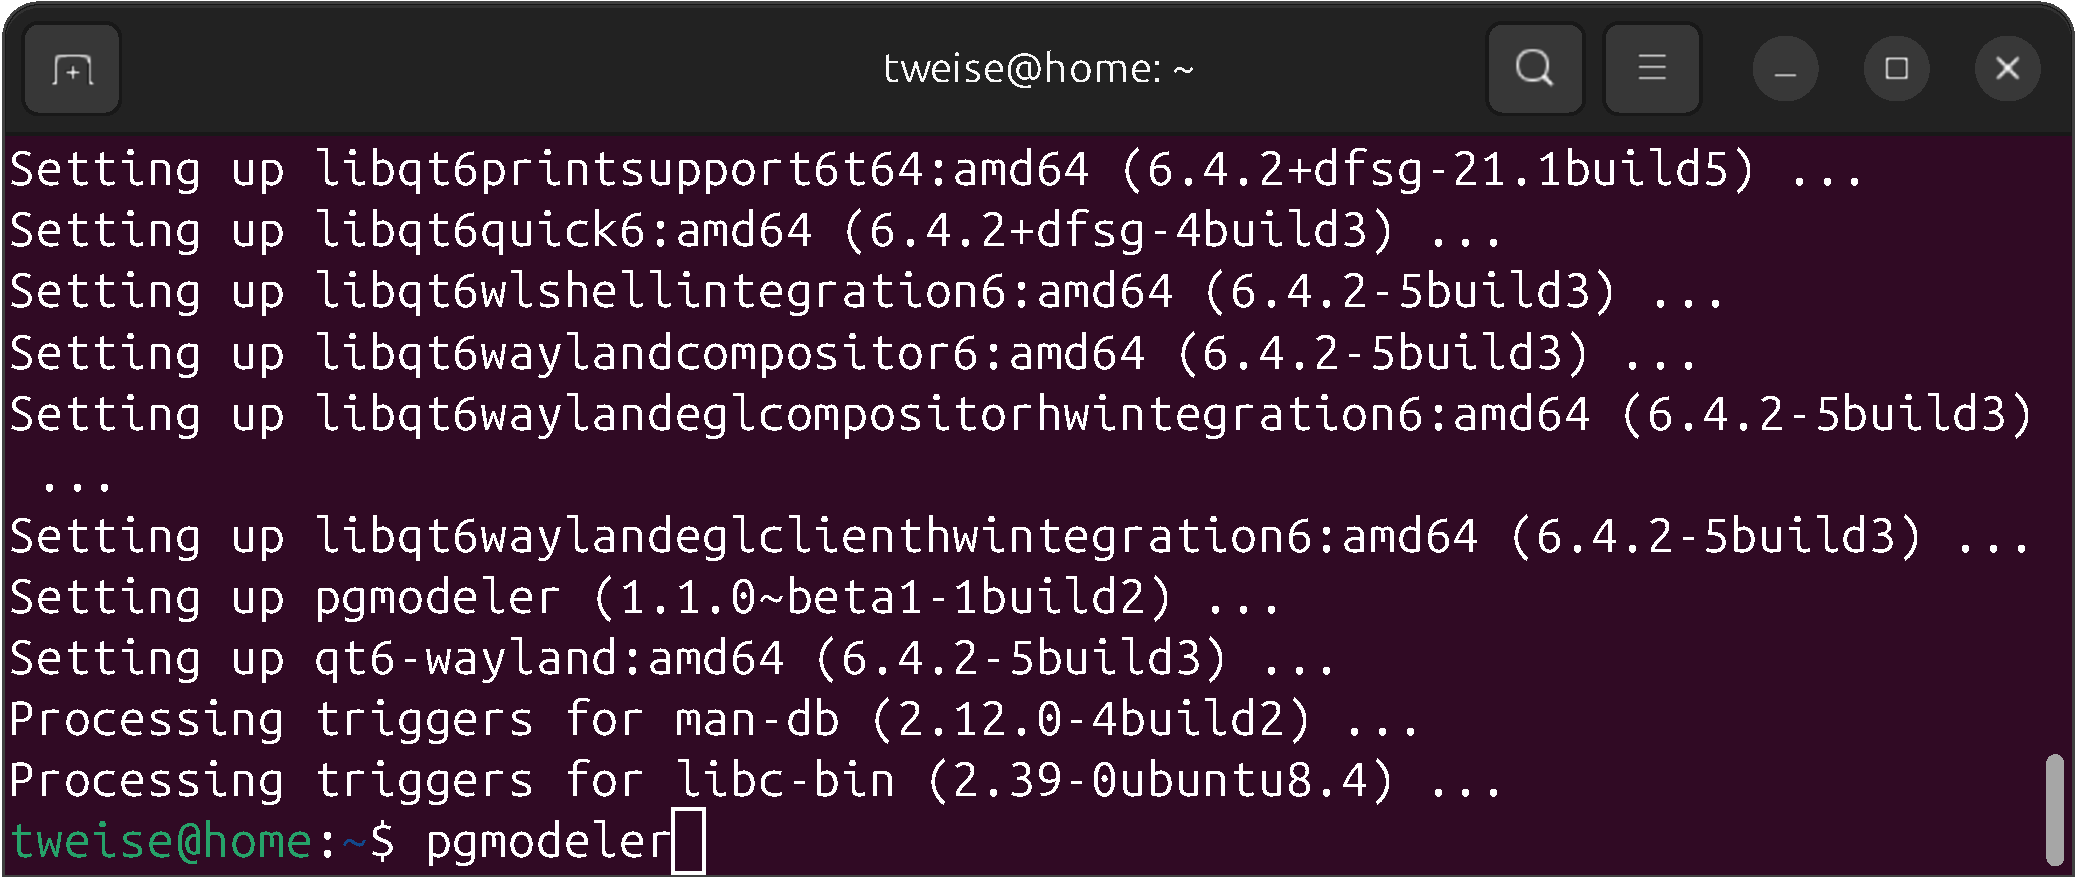
\includegraphics[width=0.7\linewidth]{\currentDir/installingPgmodelerUbuntu06run}}%
%
\floatRowSep%
%
\subfloat[][%
The program may or may not display an error notification window. %
If this notification pops up, we can simply ignore it and click on~\menu{OK}.%
\label{fig:installingPgmodelerUbuntu07error}%
]{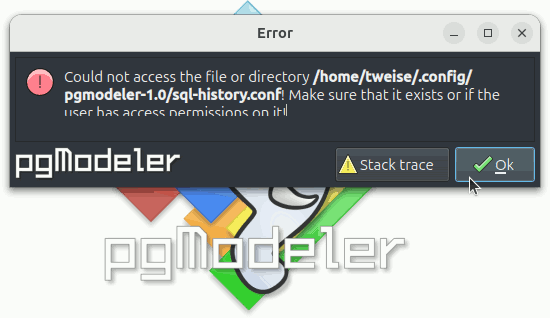
\includegraphics[width=0.6\linewidth]{\currentDir/installingPgmodelerUbuntu07error}}%
%
\caption{The installation steps for \pgmodeler\ under \ubuntu\ \linux~(continued).}%
\label{fig:installingPgmodelerUbuntu:B}%
\end{figure}%
%
\begin{figure}%
\ContinuedFloat%
\centering%
%
\subfloat[][%
The \pgmodeler\ window opens.%
\label{fig:installingPgmodelerUbuntu08open}%
]{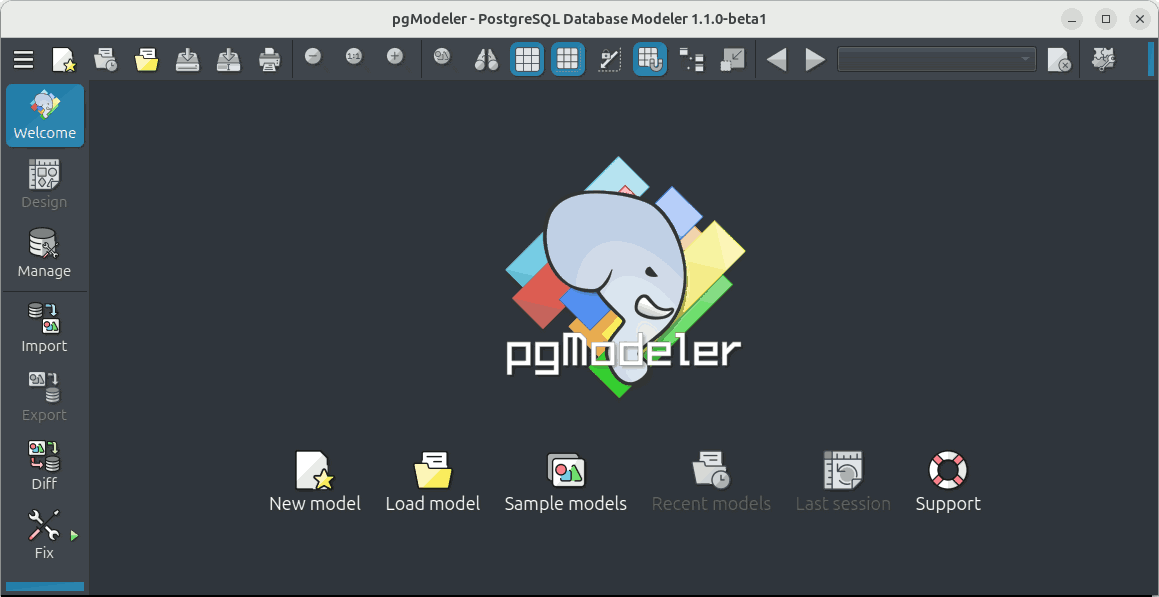
\includegraphics[width=0.7\linewidth]{\currentDir/installingPgmodelerUbuntu08open}}%
%
\floatRowSep%
%
\subfloat[][%
For this book, I will use the \pgmodeler\ in light mode, so we click on \menu{\pgmodelerMainMenu>Edit>Settings}.%
\label{fig:installingPgmodelerUbuntu09openSettings}%
]{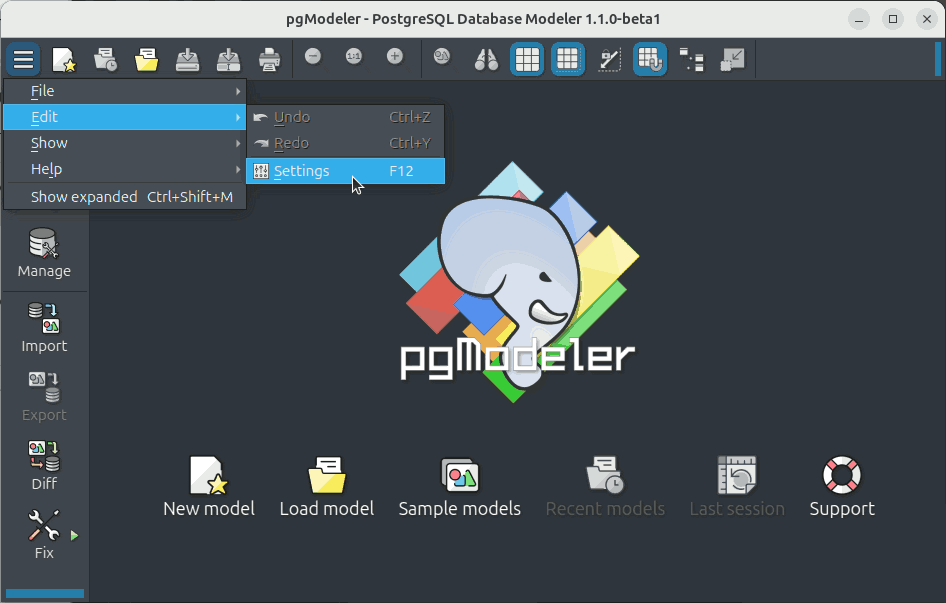
\includegraphics[width=0.7\linewidth]{\currentDir/installingPgmodelerUbuntu09openSettings}}%
%
\floatRowSep%
%
\subfloat[][%
In the \menu{Appearance} menu, we change the theme the \menu{Light}{\dots}%
\label{fig:installingPgmodelerUbuntu10themeLight}%
]{\tightbox{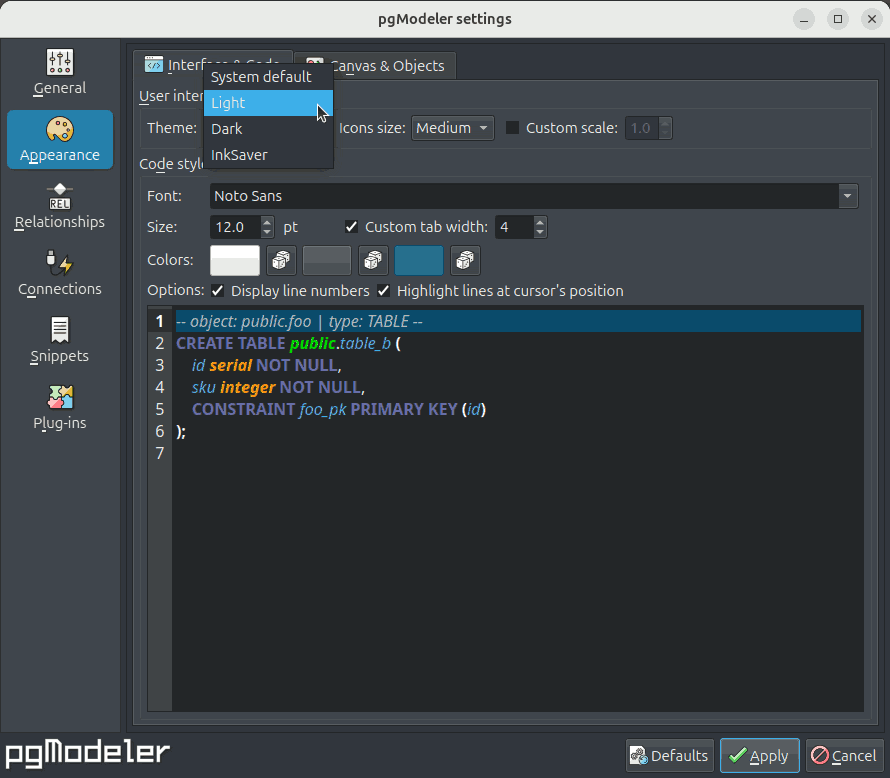
\includegraphics[width=0.45\linewidth]{\currentDir/installingPgmodelerUbuntu10themeLight}}}%
%
\floatSep%
%
\subfloat[][%
{\dots}and click on \menu{Apply}.%
\label{fig:installingPgmodelerUbuntu11themeLightSet}%
]{\tightbox{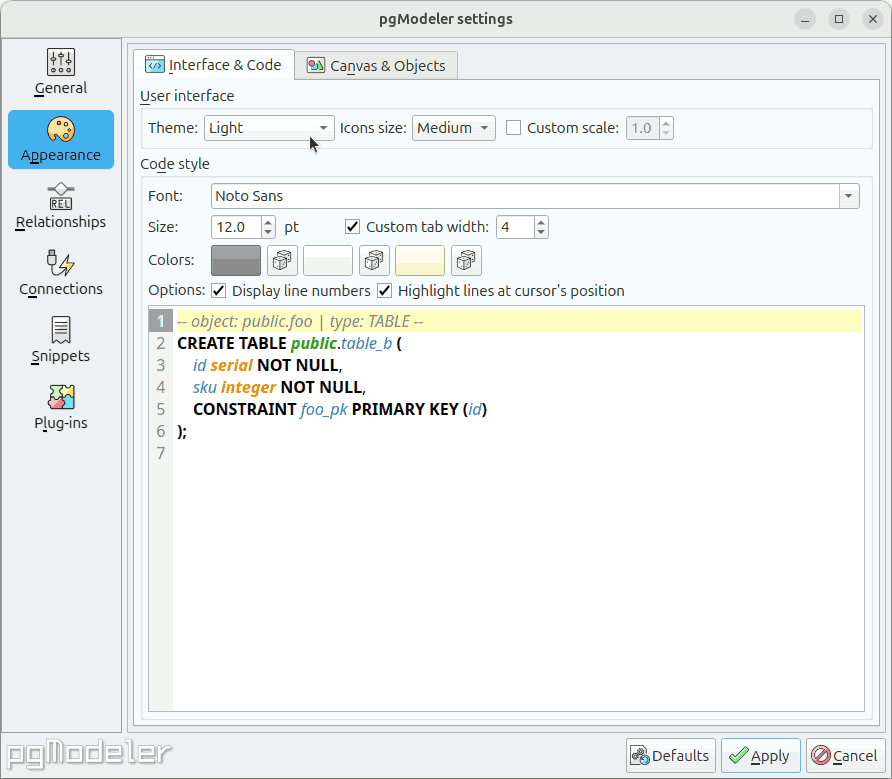
\includegraphics[width=0.45\linewidth]{\currentDir/installingPgmodelerUbuntu11themeLightSet}}}%
%
%
\caption{The installation steps for \pgmodeler\ under \ubuntu\ \linux~(continued).}%
\label{fig:installingPgmodelerUbuntu:C}%
\end{figure}%

\begin{figure}%
\ContinuedFloat%
\centering%
%
\subfloat[][%
In the \menu{Relationships} register, we make sure that the connection mode is set to \inQuotes{Crow's foot notation.}%
\label{fig:installingPgmodelerUbuntu12connectionMode}%
]{\tightbox{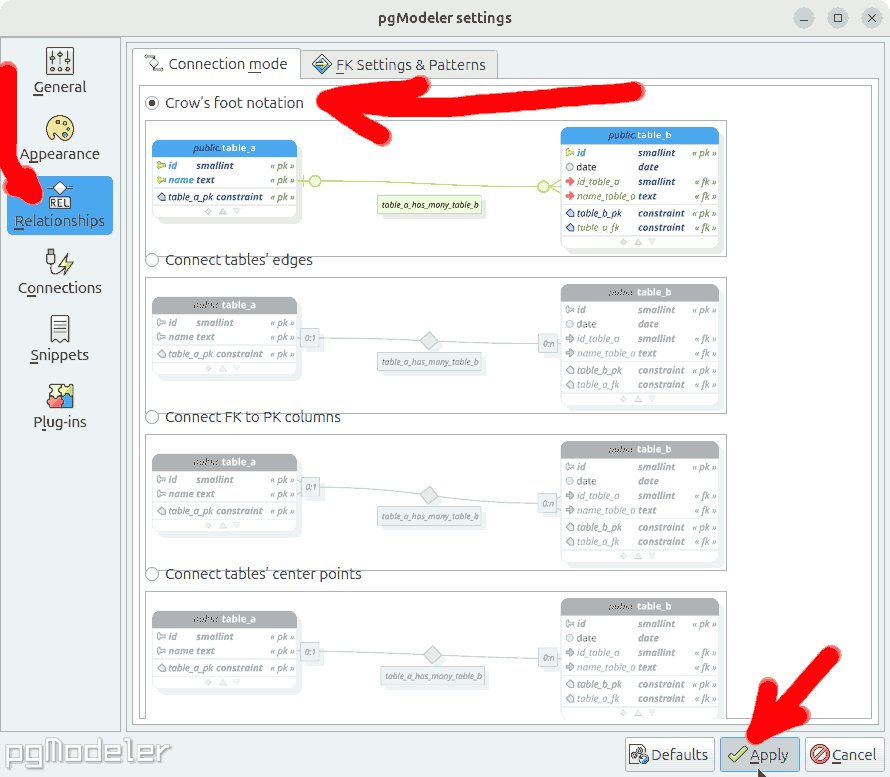
\includegraphics[width=0.45\linewidth]{\currentDir/installingPgmodelerUbuntu12connectionMode}}}%

\caption{The installation steps for \pgmodeler\ under \ubuntu\ \linux~(continued).}%
\label{fig:installingPgmodelerUbuntu:D}%
\end{figure}%
%
Under \ubuntu\ \linux, we can install the \pgmodeler\ via \bashil{apt-get}.
We therefore first open a \bash\ \pgls{terminal} via \ubuntuTerminal.
In \cref{fig:installingPgmodelerUbuntu01aptGetInstall}, we then type in \bashil{sudo apt-get install pgmodeler} and hit~\keys{\return}.
Installing software this way requires the \pgls{sudo} permission.
In \cref{fig:installingPgmodelerUbuntu02pw}, we thus get asked for the \pgls{sudo} password.
We type it in, and hit~\keys{\return}.

The system now tells us the packages that need to be installed and asks us whether we are OK with that.
We are, because we need the \pgmodeler.
So we type~\keys{Y} and hit~\keys{\return} in \cref{fig:installingPgmodelerUbuntu04yny}.%
In \cref{fig:installingPgmodelerUbuntu05installed}, the \pgmodeler\ gets downloaded and installed.

After the installation is completed, we can run the \pgmodeler\ by typing \bashil{pgmodeler} into the \bash\ \pgls{terminal} and hitting~\keys{\return} in \cref{fig:installingPgmodelerUbuntu06run}.
The \pgmodeler\ will start up.
Usually only at the first time you start it, it may or may not display an error notification window as shown in \cref{fig:installingPgmodelerUbuntu07error}.
If this notification pops up, we can simply ignore it and click on~\menu{OK}.

The \pgmodeler\ window opens in \cref{fig:installingPgmodelerUbuntu08open}.
For this book, I will use the \pgmodeler\ in light mode.
If you also want to use the light mode, you would click on \menu{\pgmodelerMainMenu>Edit>Settings}, as shown in \cref{fig:installingPgmodelerUbuntu09openSettings}.
In the \menu{Appearance} menu, we change the theme the \menu{Light} in \cref{fig:installingPgmodelerUbuntu10themeLight}.
We then click on \menu{Apply} in \cref{fig:installingPgmodelerUbuntu11themeLightSet}.
Then, in the \menu{Relationships} register, we make sure that the connection mode is set to \inQuotes{Crow's foot notation,} as shown in \cref{fig:installingPgmodelerUbuntu12connectionMode}.
The \pgmodeler\ is now installed and ready to use.%
\FloatBarrier%
\endhsection%
%
